\documentclass[12 pt]{article}
\usepackage[utf8]{inputenc}
\usepackage{graphicx}
\usepackage{amsmath}
\usepackage[version=4]{mhchem}
\usepackage{siunitx}
\usepackage{longtable,tabularx}
\usepackage{float}
\usepackage[left=1in, right=1in]{geometry}

\title{AEEM5063 HW\#1}
\date{09.11.24}
\author{Slade Brooks \\ M13801712}

\begin{document}
\maketitle

The International Space Station (ISS) is commonly referred to as a ``weightless environment''. However, as shown in
Figure~\ref{fig:grav}, the acceleration due to gravity is still almost 90\% of its value at sea level at the 400~km
orbit of the ISS.
\begin{figure}[H]
    \centering
    \includegraphics[width=0.7\linewidth]{figs/grav.png}
    \caption{Plot of acceleration due to gravity across a range of altitudes [1].}
    \label{fig:grav}
\end{figure}
Despite the acceleration due to gravity being similar, it can be seen from videos of the ISS that the astronauts are in
a ``zero-g'' environment and are able to float. This is due to the ISS being in free fall. ``The condition of
microgravity comes about whenever an object is in free fall'' [2]. The ISS is constantly falling towards the Earth in
its orbit, causing a constant free fall. ``Astronauts feel weightless when there is nothing opposing the force of
gravity''---the normal force that we feel when not in free fall is what allows us to perceive weight as we know it [3].
Typically, when sitting in a chair or standing on the ground, there is a normal force acting on our body that opposes
the force of gravity. We either feel the chair or ground pushing back against us. In free fall, this feeling is no
longer there. With no normal forces acting on any objects, they appear to float. Astronauts feel weightless because the
sensation of weight is created by the normal force, not the force of gravity. The free fall of the ISS is different than
the free fall of a parachuter jumping out of a plane. The ISS has no forces acting on it other than gravity---a true
free fall [4]. While sometimes referred to as free fall, a parachuter also feels aerodynamic drag acting on them, and thus
do not feel weightless. \par
Being in orbit allows for an object to experience free fall and in turn zero gravity. Orbit is achieved when an object
is moving at the correct speed to ``miss'' an object it is falling towards. Objects ``fall around'' Earth (or any object
they are orbiting) when they are travelling at the proper speed for orbit. Figure~\ref{fig:sat} shows a diagram of an
object in orbit and the direction its velocity and forces are in. Gravity pulls the object towards Earth, but its
velocity tangential to its path around Earth keeps it from truly reducing its height. This allows it to follow a
circular trajectory around the body is it orbiting. There are no external forces required once an object is in orbit.
Typically, an object like a satellite would be placed into its desired orbit by a rocket engine, but once it has reached
the desired orbital altitude and the corresponding speed, it will no longer require any external forces besides gravity
to maintain orbit.
\begin{figure}[H]
    \centering
    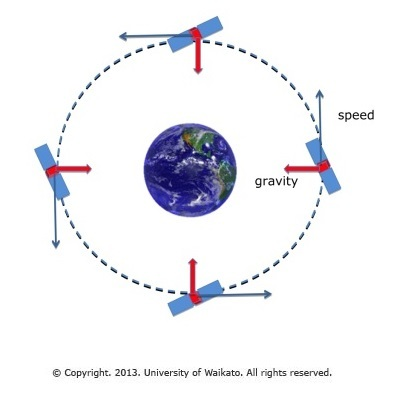
\includegraphics[width=0.5\linewidth]{figs/sat.jpg}
    \caption{Satellite speed and force directions [5].}
    \label{fig:sat}
\end{figure}
Being in orbit allows for the true free fall condition to be satisfied regardless of the orbital altitude. As long as an
object is in orbit, the only force acting on it will be gravity, and it will be weightless. This explains why the ISS
feels 90\% of the Earth's gravity but can still be a zero g environment. If it were possible, an object orbiting at sea
level would still feel weightless, even though it was feeling 100\% of the Earth's gravity.

\pagebreak
\section*{Citations}
1. Lecture Slides, ``Astrodynamics\_Lesson02\_Kim'', slide 11. \\
2. NASA, ``What is Microgravity'', 02.13.2009,
\begin{verbatim}
https://www.nasa.gov/centers-and-facilities/glenn/what-is-microgravity/#:~:text=But%20
they're%20not%20falling,immediately%20starts%20falling%20towards%20Earth.
\end{verbatim}
3. Lisa Heppler, ``Free Falling: the science of weightlessness'', 10.18.2023,
\begin{verbatim}
    https://sitn.hms.harvard.edu/flash/2018/free-falling-the-science-of-weightlessness/
\end{verbatim}
4. Wikipedia, ``Free fall'',
\begin{verbatim}
    https://en.wikipedia.org/wiki/Free_fall
\end{verbatim}
5. Science Learning Hub, ``Gravity and satellite motion'',
\begin{verbatim}
    https://www.sciencelearn.org.nz/resources/268-gravity-and-satellite-motion
\end{verbatim}

\end{document}